
\begin{figure}[t!]
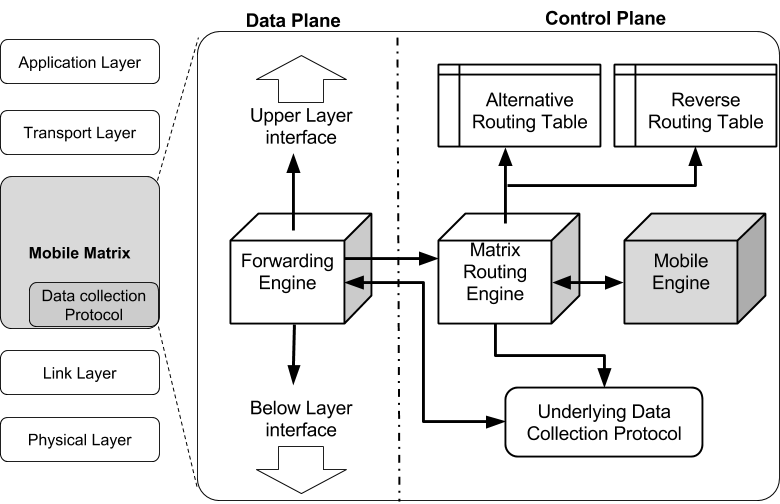
\includegraphics[width=\linewidth]{img/matrix-architecture-v3}
\caption{$\mu$Matrix protocol's architecture.}
\label{fig:architecture}
\end{figure}

\section{Design Overview}
\label{sec:design}

$\mu$Matrix enables any-to-any communication for mobile and static nodes in 6LoWPANs. $\mu$Matrix manages mobile nodes without changing its IPv6 address. Also, the protocol preserves all features from previous implementation (such as memory efficiency and fault tolerance)~\cite{Peres:2016}. 
Figure~\ref{fig:architecture} presents the protocol's architecture. $\mu$Matrix lies at network layer with an underlying data collection protocol (such as CTP or RPL). $\mu$Matrix has two planes: 
\begin{inparaenum}[i)]
  \item \textbf{Control plane} able to split and distribute the available address space, manage route tables, and handle mobile nodes;
  \item \textbf{Data plane} capable on querying route tables and forward data and control packets.
\end{inparaenum}
 
$\mu$Matrix operation consists of the following phases:  

\noindent \textbf{1. Collection tree initialization (Ctree):} An underlying routing protocol (e.g CTP~\cite{ctptosn2014} or RPL~\cite{lee2012rpl}) creates a collection routing tree.
    
\noindent \textbf{2. Descendants convergecast, IPv6 tree:} once the collection tree is stable, $\mu$Matrix builds an address hierarchy tree (IPtree) by using MHCL algorithm~\cite{Peres:2016, PeresG16:2016}. Initially, IPtree has the same topology as Ctree$^R$ (top-down direction), but in runtime, they may differ.

\noindent \textbf{3. Mobility management:} $\mu$Matrix manages the RCtree structure, a tree that reflects the topology changes due to nodes mobility.

\noindent  \textbf{4. Standard routing:} bottom-up routing follows the Ctree built in phase 1, while top-down the IPtree. Any-to-any routing combines both previous schemes, i.e., a packet flows bottom-up fashion until a Least Common Ancestor (LCA) between the sender and receiver and then it flows top-down until the destination.

\subsection{Mobility detection}
\label{subsec:reverse-tt}

Mobility detection is a key issue to handle mobile nodes on $\mu$Matrix. If nodes by itself inform its motion (e.g. by using accelerometer or GPS) to the protocol, then we refer to as active motion, otherwise if the protocol infer the node movement, we refer to passive motion.

Trickle~\cite{Levis:2004} algorithm passively detects topology changes. However, Trickle lacks in agility to detect changes in dynamic network and mobile nodes. We propose Reverse Trickle timer that operates similarly to the standard algorithm, but in reverse order. 

\begin{figure}[t!]
\centering
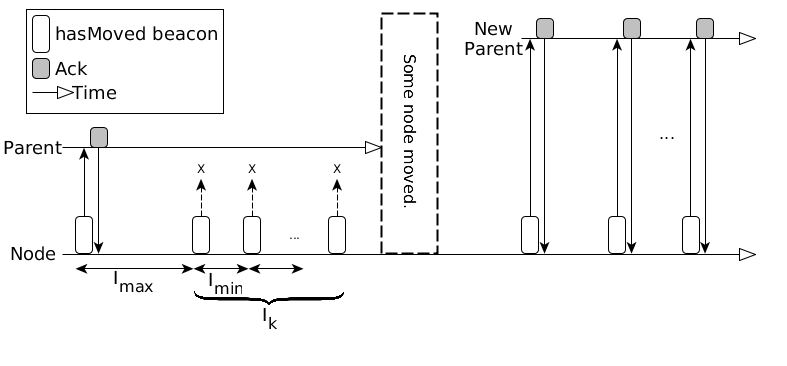
\includegraphics[width=1\linewidth]{img/reverse-tt}
\caption{Reserve Trickle timer operation.}
\label{fig:reverse-TT}
\end{figure}

Reverse Trickle introduce a control message and three parameters: 
\begin{inparaenum}[i)]
    \item \texttt{hasMoved} beacon;
    \item $I_{max}$ and $I_{min}$ the maximum and minimum time interval to send a \texttt{hasMoved} beacon;
    \item $I_k$ the number of attempts to query a node before declaring a inconsistency.
\end{inparaenum}
These parameters must defined by the network operator before.

Figure~\ref{fig:reverse-TT} shows the Reverse Trickle procedure. First, a node starts sending unicast \texttt{hasMoved} beacons to its parent. $I_{max}$ is the interval between two consecutive \texttt{hasMoved}. If the node did not receive an ack for a \texttt{hasMoved} beacon, then it sets the interval to $I_{min}$. After $I_k$ unsuccessful attempts, the node knows that someone moved. Thus, the node can take actions, for example, properly perform a handover to another parent and then the procedure restarts. Note that by setting the Reverse Trickle parameters, the network operator should consider the trade-off between delay to detect mobility and number of beacons. For a smaller delay to mobility detection, $I_{max}$ must be tuned to small values at cost of more \texttt{hasMoved} beacons. In our experiments (Section~\ref{sec:evaluation}) reverse trickle parameters were set according to application data rate (Table~\ref{tab:sim-params}). 

In \cite{oliveira2016low}, the authors argue that a common modification to support mobility is change the control message periodicity. The typical approach uses a simple periodic timer or the standardized Trickle timer. While reverse trickle waits for $I_{max} + T_k \times I_{min}$ to detect a topology change, where $I_{min} \ll I_{max}$, the periodic and standardized Trickle approaches wait for at least $2\times I_{max}$.  

\subsection{Control Plane}
\label{subsec:control-plane}

\tikzset{
    simpleNode/.style={
        circle,very thick,minimum size=6mm,
        draw=black!50, top color=white,bottom color=black!20,font=\ttfamily,
        align=center
    },
    rootNode/.style={simpleNode,
        % The shape:
        rectangle, rounded corners=0,minimum size=6mm,
        % Font
        font=\ttfamily},
    nilNode/.style={},
    emphGrayEdge/.style={edge from parent/.style={dashed,gray,draw}},
    emphRedEdge/.style={edge from parent/.style={solid,red, very thick, draw}},
    normEdge/.style={edge from parent/.style={solid,black,thin,draw}},
    normDashedEdge/.style={edge from parent/.style={dashed,black,thin,draw}}
}

\begin{figure}[!ht]
\setlength\belowcaptionskip{-5ex}
\begin{center}
    \subfigure[Ctree structure, ID inside the nodes.]
    {
        \begin{tikzpicture}[ <-,>=stealth',shorten >=1pt,auto,semithick,transform shape,
       level/.style={sibling distance=10mm, level distance = 1.2cm}]
        
        \node [rootNode] (Root) {1}
            child{ node [simpleNode] (2) {2} 
                    child{ node [simpleNode] (5) {5}
                            child[dashed]{node [] (7) {}}
                            child[dashed]{node [] (8) {}}}
                    child{ node [simpleNode] (6) {6}
                            child[dashed]{node [] (9) {}}}}
            child{ node [simpleNode] (3) {3} }
            child{ node [simpleNode] (4) {4} 
                    child[dashed]{node [] (10) {}}}
            ;
            
        \node[draw, align=left] at (0.8,-3.3) 
                {
                \textbf{Ctree}
                };
        \end{tikzpicture}
    }
    \,
    \subfigure[IP addres assignment by MATRIX hierarchical distribution. Simplified 8-bit IP inside the nodes.]
    {
        \begin{tikzpicture}[ ->,>=stealth',shorten >=1pt,auto,semithick,transform shape,
       level/.style={sibling distance=10mm, level distance = 1.2cm}]
        
        \node [rootNode] (Root) {1}
            child{ node [simpleNode] (2) {16} 
                    child{ node [simpleNode] (5) {27}
                            child[dashed]{node [] (7) {}}
                            child[dashed]{node [] (8) {}}}
                    child{ node [simpleNode] (6) {152}
                            child[dashed]{node [] (9) {}}}}
            child{ node [simpleNode] (3) {184} }
            child{ node [simpleNode] (4) {208} 
                    child[dashed]{node [] (10) {}}}
            ;
            
        \node[draw, align=left] at (0.8,-3.3) 
                {
                \textbf{IPtree}
                };
        \end{tikzpicture}
    }
 
    \subfigure[Node 2 moves, then Ctree changes.]
    {
        \begin{tikzpicture}[<-,>=stealth',shorten >=1pt,auto,semithick,transform shape,
           level/.style={sibling distance=9.5mm, level distance = 1.2cm}]
        
        \node [rootNode] (Root) {1}
            child[emphGrayEdge]{ node [simpleNode, dashed, top color=white,bottom color=white] (2) {2}
                    child[emphGrayEdge]{ node [simpleNode, solid] (5) {5}
                            child[normDashedEdge]{node [] (7) {}}
                            child[normDashedEdge]{node [] (8) {}}
                            edge from parent [] node [left] {X}
                            }
                    child{ node [simpleNode, solid] (6) {6}
                            child[normDashedEdge]{node [] (9) {}}
                            edge from parent [] node [right] {X}
                        }
                    edge from parent [] node [above] {X}
                     }
            child{ node [simpleNode] (3) {3} }
            child{ node [simpleNode] (4) {4} 
                    child[emphRedEdge]{node [simpleNode] (new2) {2}}
                    child[dashed]{node [] (10) {}}}
            ;
        
        \draw[very thick, red] (6) -- (5); 
        \draw[very thick, red] (3) -- (6); 
        
        \node[draw, align=left] at (0.67,-3.3) 
                {
                \textbf{Ctree} \\ \textbf{\textcolor{red}{CHANGES}}
                };
        \end{tikzpicture}
    }
    \!
    \subfigure[$RCtree \cup  IPtree$. Red and thicker links are in RCtree, but not in IPtree.]
    {
        \begin{tikzpicture}[->,>=stealth',shorten >=1pt,auto,semithick,transform shape,
           level/.style={sibling distance=10.5mm, level distance = 1.2cm}]
        
        \node [rootNode] (Root) {1}
            child[color=white, text=black]{ node [color=white] (2) {2}
                    child[]{ node [simpleNode, solid] (5) {27}
                            child[normDashedEdge]{node [] (7) {}}
                            child[normDashedEdge]{node [] (8) {}}
                            }
                    child[]{ node [simpleNode, solid] (6) {152}
                            child[normDashedEdge]{node [] (9) {}}
                        }
                     }
            child{ node [simpleNode] (3) {184} }
            child{ node [simpleNode] (4) {208} 
                    child[emphRedEdge]{node [simpleNode] (new2) {16}}
                    child[dashed]{node [] (10) {}}}
            ;
        
        \draw[very thick, red] (6) -- (5); 
        \draw[very thick, red] (3) -- (6); 
        
        \node[draw, align=left] at (0.8,-3.3) 
                {
                \textbf{\textcolor{red}{RCtree $\cup$}}\\
                \textbf{IPtree}
                };
        \end{tikzpicture}
    }
    
    \caption{Routing data structures: Ctree, IPtree, and RCtree.}
    \label{fig:trees}
\end{center}
\end{figure}


\subsubsection{Routing data structures}
\label{subsubsec:controlDataStructures}

$\mu$Matrix maintains three routing trees structures:
\begin{inparaenum}[i)]
  \item \textbf{Ctree}: a collection tree built by the underlying collection protocol;
  \item \textbf{IPtree}: an IPv6 hierarchical tree created by MATRIX initialization and kept static afterward, except when new nodes join the network;
  \item \textbf{RCtree}: a tree that reflects the topology changes caused by node mobility.
\end{inparaenum}


Initially, IPtree = Ctree$^{R}$ and RCtree $= \emptyset$ (see Figures~\ref{fig:trees}(a)(b)). Whenever a topology change occurs due to mobility in Ctree, the new link is added into RCtree, and it is maintained while the change remains, therefore $RCtree = Ctree^{R} \setminus IPtree$ (see Figures~\ref{fig:trees}(c)(d)). RCtree is not essentially a tree since it contains only reversed links in Ctree but not in IPtree. Nevertheless, $RCtree \cup IPtree$ is, in fact, a tree, which $\mu$Matrix uses to downward routing. Each node $\eta$ keeps the following information to build and maintain theses trees:

\begin{itemize}
    \item $CTparent(\eta)$: the ID of the current parent of a node $\eta$ in the dynamic collection tree;
    
    \item  $PRVparent(\eta)$: the ID of $\eta$'s previous $CTparent(\eta)$;
    
    \item  $IPparent(\eta)$: the ID of the node that assigned to $\eta$ its IPv6 and IP range; %Initially $CTparent(\eta) = IPparent(\eta)$;
              
    \item  $IPchildren(\eta)$: the standard (top-down) routing table with IPv6 ranges for one-hop descendants of $\eta$ in IPtree;
    
    \item $Mtable(\eta)$: a temporary alternative routing table for mobility management. Each entry has an IPv6 range, next hop, and Time Has Lived (THL) fields.
        
\end{itemize}

$\mu$Matrix introduce one routing packet and one parameter to control exchanging topology information and maintain the $Mtables$:
\begin{inparaenum}[i)]
    \item \texttt{nodeInfo} routing frame has 7 fields: seqNum, IPv6 Node, IP range, IPv6 IPparent, CTparent, TTL, and Type. The fields are self-explanatory, except by the type field, which specifies if routing frame is a \texttt{keepRoute.\{IP\_ONLY or IP\_AND\_RANGE\}} entry insertion, or \texttt{rmRoute} to remove a entry. In the following, we will use \texttt{keepRoute} for short;
    \item \texttt{$\delta$} parameter specifies the time between sending two consecutive.
\end{inparaenum}

In mobile scenarios, a node fills $Mtable$ upon receiving \texttt{keepRoute} beacons from mobile nodes. The node keeps $Mtable$ entries as long as it receives \texttt{keepRoute}. Otherwise, it uses a $THL$ mechanism to remove entries (see Sec~\ref{subsec:memory-footprint} for memory footprint analysis). In static scenarios any node stores one-hop neighborhood information in $IPparent(\eta)$, this requires $O(k)$ entries, where $k$ is the number of node's children. This memory footprint is better than state-of-the-art, e.g., RPL would need at least $1$ routing entry for every child in a node sub-tree for top-down routing fashion

\begin{figure}[t!]
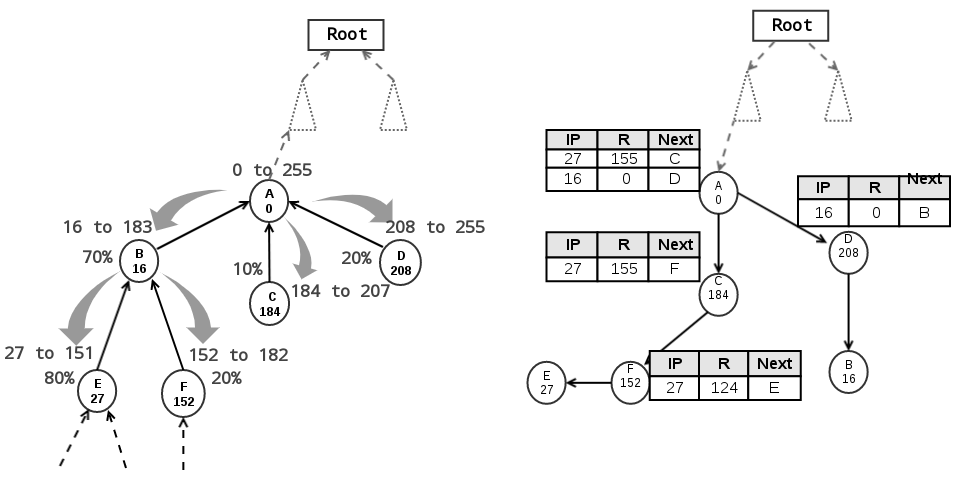
\includegraphics[width=\linewidth]{img/hierarchical-address-assignment}
\caption{Simplified hierarchical address assignment
with 8-bit available address space and \unit[6.25]{\%} of address reserve for delayed nodes. Inside the nodes its label and assigned IP, the \% next the nodes express the approximate sub-tree size. Thick downwards arrows indicates the available IP range fairly distribution.  In the rightmost, $Mtable$ after B moves.}
\label{fig:hierarchical-addr-assigment}
\end{figure}

\subsubsection{IPv6 multihop host configuration}

$\mu$Matrix relies on an underlying collection routing protocol to build the Ctree. Once the Ctree is stable\footnote{A node is stable if it reaches $k$ times the maximum maintenance beacon period of Ctree protocol without changing its parent. We use Trickle~\cite{Levis:2004} as beacon scheme.}, the address space available to the border router, e.g., the 64 least-significant bits of the IPv6 address (or a compressed 16-bit representation of the latter), is hierarchically partitioned among nodes in the Ctree. The (top-down) address distribution is preceded by a (bottom-up) convergecast phase, in which each node counts the total number of its descendants and propagates it to its parent. Thus node knows how many descendants each child has. Such information is required to distribute IP ranges in a fairly way. As result of this procedure is obtained the IPtree.

Figure~\ref{fig:hierarchical-addr-assigment} most left shows the process. First, it is created the Ctree (upwards arrows), and then, after the Ctree stabilization, the convergecast phase occurs allowing nodes to know the size of theirs sub-tree (\% next to each node). Next, the root starts the IP distribution by auto-setting its IP (e.g. the first available IP from range) and then reserving a portion of the range for delayed nodes. Next, the node distributes the remaining range fairly between its children (e.g. in Figure~\ref{fig:hierarchical-addr-assigment} B receives 70\% of available range, i.e., from 16 to 183). Finally, each node repeats the IP distribution process.


\begin{figure}[!ht]
\centering
    \begin{tikzpicture}[
        ->,>=stealth',shorten >=1pt,auto,semithick, transform shape,
        node distance=4mm and 10mm,
        nonterminal/.style={
        % The shape:
        rectangle,
        % The size:
        minimum size=6mm,
        % The border:
        very thick,
        draw=red!50!black!50, % 50% red and 50% black,
        % and that mixed with 50% white
        % The filling:
        top color=white, % a shading that is white at the top...
        bottom color=red!50!black!20, % and something else at the bottom
        % Font
        font=\itshape
        },
        terminal/.style={
        % The shape:
        rectangle,minimum size=6mm,rounded corners=3mm,
        % The rest
        very thick,draw=black!50,
        top color=white,bottom color=black!20,
        font=\ttfamily}]
        
        % \node (HL) [initial, accepting, nonterminal,initial text=] {HL};
        % \node (NM) [terminal,above right=of HL]         {NM};
        % \node (PM) [terminal,below right=of HL]         {PM};
        % \node (SM) [terminal,below right=of NM]         {SM};
        \node (HL) [initial, accepting, nonterminal,initial text=] {HL};
        \node (SM) [terminal, right=of HL]         {SM};
        \node (NM) [terminal,above right=of SM]         {NM};
        \node (PM) [terminal,below right=of SM]         {PM};
         
        \path 
            (HL) edge   [bend left]     node {1} (SM)
            (SM) edge   [bend left]     node {5} (HL)
            (SM) edge   [bend left]     node [pos=0.7, sloped, above] {2} (PM)
            (PM) edge   [bend left]     node [pos=0.5, sloped, below] {4} (SM)
            (SM) edge   [bend right]    node [pos=0.7, sloped, below] {3} (NM)
            (NM) edge   [bend right]    node [pos=0.5, sloped, above] {4} (SM)
            % (NM) edge   [bend right]    node [below] {5} (HL)
            % (PM) edge   [bend left]     node [above] {5} (HL)
            ;
        
        \node[draw] at (-2.5,0) 
        {
        \tiny
        \begin{tabular}{cl}
        HL & Home Location \\
        SM & Someone Moved \\
        NM & Node Moves \\
        PM & Parent Moves \\
        \hline	
        1 & IPparent does not answer \\
        2 & Children are active \\
        3 & Children are NOT active \\
        4 & CTparent does not answer \\
        5 & IPparent is back \\
        \end{tabular}
        };
    \end{tikzpicture}
\vspace{-0.4cm}
\caption{Mobile Engine state machine.}
\label{fig:mobile-engine-state-machine}

\end{figure}

\subsubsection{Mobility management}

After host configuration, $\mu$Matrix starts the mobile engine allowing nodes to move around the 6LoWPAN. Mobile engine uses a finite state machine (Figure~\ref{fig:mobile-engine-state-machine}). Each node can be in one state depending on its previous condition and the knowledge about its neighborhood. The engine also uses Reverse Trickle to recognize mobility and transit among states. In the following, we discuss the actions taken in each of those states.  

Each node begins at Home Location (HL) state. In HL, the nodes start the reverse trickle with its $CTparent(\eta)$ (initially, $CTparent(\eta) = Pparent(\eta)$ see Figure~\ref{fig:node-static}). When reverse trickle identifies a mobility event, then the node transit to Someone Moved (SM) state.

When a node is at SM state, it knows that someone moved, but it does not know if itself or its parent moved. There are at last two ways to automatically find out who moved. First, a node pro-actively queries its children ($IPChildren(\eta)$), if no one answer then the node moved; otherwise the parent moved. Second, a node must wait for a period (e.g. one $I_{max}$) to receives \texttt{hasMoved} beacons from its children and then infer who moved. We use the second approach in our implementation. After discovering who moved, the node goes to Node Moved (NM) or Parent Moved (PM) state. 

Several actions are taken when a node reaches NM state. Firstly, the node disables the  $IPChildren(\eta)$ table due to the node new position in the Ctree. Next, the $Mtable$ is cleaned, because it must be outdated. Then, the node triggers the new parent discovery from underlying collection protocol. When the node is attached again to the Ctree, it restarts reverse trickle with new CTparent and begins sending \texttt{keepRoute.IP\_ONLY} at a frequency of $\delta$ to its IPparent.  Figure~\ref{fig:movement-cases}(a)(b) shows this situation. When B sends \texttt{keepRoute} beacons to A, when B moves and find a new CTparent. The beacons travel upward to the LCA(A, B) and then downwards to the node A.  

When a node reaches PM, this means that its parent moved. Then, the node triggers the parent discovery mechanism. When it is attached again to Ctree, it restarts the reverse trickle and begins sending two \texttt{keepRoute} beacons (if it has children the beacon contains \texttt{IP\_AND\_RANGE}, otherwise \texttt{IP\_ONLY} ) at a frequency of $\delta$ to IPparent and its grand IPparent. Figure~\ref{fig:movement-cases}(c)(d) illustrate this situation. If B moves, then C eventually reaches PM state, and then C begins sending \texttt{keepRoute} beacons to its $grandIPparent = A$. The messages travel to LCA(A, C) and then to the ultimate destinations. 

Eventually, nodes return to their home position being attached again to its IPparent in Ctree. This situation also triggers some actions. First, the node stops to sending \texttt{keepRoute} beacons and sends to its very previous CTparent = PRVparent a \texttt{rmRoute} containing its information to properly remove outdated routes nodes' $Mtable$. Also, the returned node restarts the reverse trickle with its IPparent.

Optional features are made to improve the mobile node management. Note that if a node is attached to a sequence of CTparent before returning to home location, then several states will be installed in the network. Although the $Mtable$' THL field exists to remove inconsistent entries, it is possible to send \texttt{rmRoute} beacons to each node' PRVparent to eliminate such inconsistency.

\begin{figure}[!t]
\begin{center}
    \subfigure[$\mu$Matrix in a static situation before B (at HL state) moves.]
    {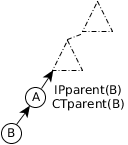
\includegraphics[width=.35\linewidth]{img/leaf-move-1}
    \label{fig:node-static}}
    \quad 
    \subfigure[B moves, then it transit to NM state and starts sending \texttt{keepRoute} beacons.]
    {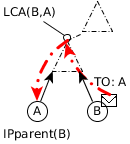
\includegraphics[width=.35\linewidth]{img/leaf-move-2}
    \label{fig:leaf-moves-2}}
    
    \subfigure[B a non leaf node before move.]
    {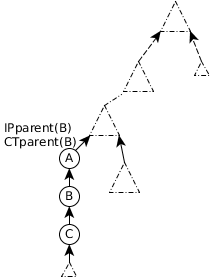
\includegraphics[width=.45\linewidth]{img/nonleaf-move-1}
    \label{fig:nonleaf-move}}
    \, 
    \subfigure[B moves, then C transits to PM state and start sending \texttt{keepRoute} beacons.]
    {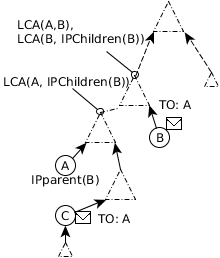
\includegraphics[width=.45\linewidth]{img/nonleaf-move-2}
    \label{fig:nonleaf-move-2}}
    
    % \vspace{-0.5cm}
    \caption{Mobile engine operation after mobility events.}
    \label{fig:movement-cases}
\end{center}
\end{figure}

\textit{Discussion:} note that a sub-tree can move and nodes still hear each other. For instance, in Figure~\ref{fig:nonleaf-move} suppose A and B move together. Then, A and C eventually will transit to PM, while B and C's sub-tree remain in HL. In this case, the LCA has two $Mtable$ entries matching with C's sub-tree, but one more restrictive than other. Thus, the LCAs play a key role, which they always route through the most restrictive $Mtable$ range match available. 

Also, note that $\mu$Matrix preserves locality when manages mobile nodes since no $MTables$ needs updates above LCA. Figure~\ref{fig:hierarchical-addr-assigment} (rightmost) illustrates this situation. When node B moves, it transits to NM state, $Mtables$ comprised in the path B to $A = IPparent(B) = LCA(B, IPparent(B))$ receive updates. B movement causes E and F to transit to PM state. Then, E and F find new routes and update the $Mtables$ between them and its grandIPparent = A. Note that $Mtable(C)$ requires only one entry for both E and F sub-trees because their IP range are contiguous and an aggregation was made.

\subsubsection{Loop avoidance}
dynamic links and mobile nodes cause topology route information to become outdated, which causes routing loops~\cite{ctptosn2014}. $\mu$Matrix uses data path validation and adaptive beaconing to detect loops CTP and RPL~\cite{ctptosn2014, lee2012rpl}. Besides that, if a node receives more than one unique control packet\footnote{Together the \texttt{keepRoute} fields (see Sec~\ref{subsubsec:controlDataStructures}) denote a unique packet instance.} in a short time, then this indicates an inconsistency in the tree, which triggers the control packet suppression and the underlying protocol route update. Also, $Mtable$ and \texttt{keepRoute} beacon have respectively Time Has Lived (THL) and Time To Live (TTL) field, which it is used to remove inconsistent routes and messages from the network.

\subsection{Data Plane: any-to-any routing}
\label{subsec:data-plane}

The Forwarding Engine (see Figure~\ref{fig:architecture}) is responsible for data forwarding. Any-to-any routing combines bottom-up forwarding, until the LCA between the sender and receiver, and then top-down forwarding to the destination. Upon receiving a data packet, the node checks if the message is for itself.
Second, the node tries to match the destination with an entry $Mtable$. Third, if any $Mtable$ entries match with the target address, then the node checks if the packet destination falls within some range in $r \in IPchildren(\eta)$, if positive match, then the node forwards the packet downwards according. Finally,  if all previous attempts fail, then the node sends the packet upwards using $CTparent(\eta)$.